\section{Proposed corrections and research-status updates}
\label{cont:sec:editorial}

The audit found a logical overstatement in the rank-conjecture
paragraph and a duplicated citation. The more substantial revisions
concern research status and the range of validity of an argument.
No counterexample was found to the stated fixed-$m$ moment theorems
or to the complex-algebra distribution theorems examined here.
The following changes are proposed for editorial integration.

\subsection{The rank-difference statement is a consequence}

In \src{chapters/05-signed-kernels.tex}, for odd $w\ge3$, the two
conjectured ranks are
\[
 \operatorname{rank}A_w=5w-6,\qquad
 \operatorname{rank}A_w^{\neg g}=\frac{9w-11}{2}.
\]
Let $V$ be the row space and let $\pi$ project onto the
non-Gaussian columns. The exact linear-algebra identity is
\begin{equation}\label{cont:eq:rank-difference}
 \dim\ker(\pi|_V)
  =\operatorname{rank}A_w-\operatorname{rank}A_w^{\neg g}.
\end{equation}
Thus the two rank formulas imply the stated Gaussian-supported
dimension $(w-1)/2$. That dimension alone fixes their difference,
and does not determine both ranks separately. The word
``Equivalently'' should therefore be replaced by an implication,
unless a separately established individual-rank statement is supplied.
This correction is also recognized in the incoming rank work
\cite{cont:RankIncoming,cont:FormalIncoming}; it is carried forward
here, not presented as a new mathematical discovery.

There is a more useful final editorial step than merely fixing this
word: integrate one of the already supplied all-weight rank proofs,
retain its exact matrix convention and certificate, and change the
conjecture to a theorem with appropriate provenance. The incoming
level-four article proves both odd-weight ranks and the even-weight
formulas. The present article does not repeat that substantial proof.

\subsection{A duplicate citation}

The proof in \src{chapters/04-proportional-depth.tex} cites DLMF
Section~2.3(iii) twice consecutively for the same invocation of
Laplace's method. One citation suffices. The accompanying
\src{editorial/proposed_corrections.patch} makes this change and the
minimal logical correction above against the pinned source.
It deliberately leaves a conjecture labelled as such until its
existing incoming proof is integrated.

\subsection[The S6 entry should have one identity and two coordinates]{The $S_6$ entry should have one identity and two coordinates}

The two candidates reconciled in Section~\ref{s6audit:sec:main}
should share one conjecture label, with
\eqref{s6audit:eq:coordinate} as the proved change of coordinates.
Keep the numerical evidence attached to the candidate it actually
tests, and cross-reference the equivalent form. The disappearance of
$G\zeta(5)$ in the second presentation is an exact shuffle
cancellation; it does not constitute independent evidence for a
second relation. The incomplete modular search in this article
provides neither a proof nor an obstruction.

\subsection{Uniformity and integral-coordinate qualifications}

The new harmonic theorem resolves the outstanding unbounded-ratio
saddle problem, but its asymptotic parameter is still $p\to\infty$.
Retain the fixed-$p$ endpoint theorem. When interpreting the old
large-$\alpha$ rate expansion, keep the actual first-pole condition
$p/h-\log h\to+\infty$ distinct from merely $p/h\to\infty$.

The reflected-moment transition explicitly shows why one cannot
substitute $m=m(n)$ into a fixed-$m$ relative error without proof.
This is a limitation already respected by the pinned theorem, not
a contradiction to it. After integration, the remaining uniform
problem should concern the bridges between the proved joint regimes
and the interaction with optimal truncation when $m$ also grows.

For distribution modules, retain the distinction between the free
full quotient $U_q$ and the image of its primitive grid. At level
fifteen, ordinary weights give primitive rank seven over
$\mathbb Q$ and five over $\mathbb F_2$, while $U_{15}$ has rank
eight over both fields. A character diagonalization which divides
by a group order cannot simply be reduced modulo a prime dividing
that order. The integral presentation supplies the needed replacement.
The baseline complex-algebra hypothesis was explicit and correct.

The spectral conventions also need to remain visible: Hurwitz
multiplication has $t_p=p^s$, whereas polylogarithm multiplication
has $t_p=p^{1-s}$. Thus the ordinary weight $t_p=1$ corresponds
respectively to $s=0$ and $s=1$. At a pole, combine the complete
meromorphic identity before taking a limit; a coefficient that
vanishes at the pole can still contribute a finite term.

\section{Reproducibility and the meaning of the computations}
\label{cont:sec:verification}

The supplementary code is organized by theorem, with small
machine-readable outputs beside the programs. Exact symbolic
calculations are separated from floating-point quadrature.
All finite checks are reproducible from the delivered archive;
the large inconclusive $S_6$ search matrix is excluded.

\subsection{Exact identities and finite algebra}

\begin{itemize}[leftmargin=*]
\item \src{code/harmonic/compile_inverse.py} regenerates the kernel
and forward transition polynomials and derives $Q_0,Q_1$ by
exact symbolic inversion. It verifies the two coefficients in the
original normalized expression as well as the logarithmic
calculation. \src{code/gaussian/audit_inverse_q1.py} independently
starts from shifted gamma cumulants and returns the same result.

\item The moment scripts derive $P_1,P_2$ twice: directly from
the centered gamma expectation and from finite offset-residue
identities. The results agree symbolically. The finite all-orders
generator produces generic $P_0,\ldots,P_3$ by default and verifies
the degree bounds. These coefficients use symbols for the local
analytic germs, so their dependence can be inspected before
substituting gamma and zeta constants.

\item \src{code/distribution/verify_integral_distribution.py}
checks complete polynomial normal-form identities at every level
$2\le q\le60$, nineteen symbolic primitive determinants,
112 finite-characteristic resolutions, and 504 complete two-prime
Smith specializations. It checks the three displayed level-fifteen
coefficient tuples over $\mathbb Q$. These finite tests check an
implementation; the all-level and arbitrary-ring assertions follow
from the finite-resolution and cycle proofs.

\item \src{code/gaussian/verify_s6_equivalence.py} uses only
Python's integer and rational arithmetic. It reconstructs the two
binomial shuffle rows, verifies the exact residual combination,
and verifies direct elimination of $g_{2,5}$. It does not evaluate
or prove the common $S_6$ conjecture.
\end{itemize}

\subsection{The exact interval step in the slope-ratio theorem}

The monotonicity theorem in Section~\ref{gs:sec:main} has a different
computational status from the diagnostic tables. Its middle-interval
inequality is a finite part of the proof. The program
\src{code/moments/certify_gamma_saddle.py} uses only integers and
rationals. It independently encloses $\gamma$, the required zeta
values, and logarithms; bounds all differentiated Taylor tails;
and evaluates entire rational subintervals with outward rounding.
The article specifies every series, remainder and interval endpoint.
The certificate covers the compact interval completely, and
analytic estimates handle the two endpoints. A second inspection
and replay produced the identical rational bound. This is an exact
computer-assisted proof, not evidence inferred from sampled signs.

\subsection{High-precision diagnostics}

The harmonic diagnostics evaluate the exact positive integral after
centering at its saddle, at fifty working decimal digits. The test
set includes $p/h\to0$, bounded ratio, very large ratio, increasing
shift, and transition points. The inverse calculation uses the same
defining integral to locate the target fraction. The largest sampled
value of $p^2|R/\mathcal S-1-E_1/p|$ is about $0.194$; this
is a sample statistic, not a universal error constant.

The joint-moment diagnostics use eighty working digits and fifteen
pairs $(n,m)$ near three transition offsets. They integrate the
defining expression with $x=e^{-y}$, centered and standardized
around the gamma mean. Two finite integration-window choices are
compared. Their very small discrepancy is a consistency check; it
does not by itself bound all quadrature or omitted-tail error.
The proof's localization estimates and Taylor bounds establish the
asymptotic theorem independently of these diagnostics.

The level-fifteen Hurwitz example is also evaluated independently at
ninety working digits, with a largest recorded absolute discrepancy
below $2.46\cdot10^{-91}$. Its proof, however, is the exact
distribution elimination, not the small decimal residual.

Figure~\ref{cont:fig:corrections} displays the reduction in error when
successive corrections are retained. It is generated directly from
the delivered diagnostic JSON files.
\begin{figure}[htbp]
\centering
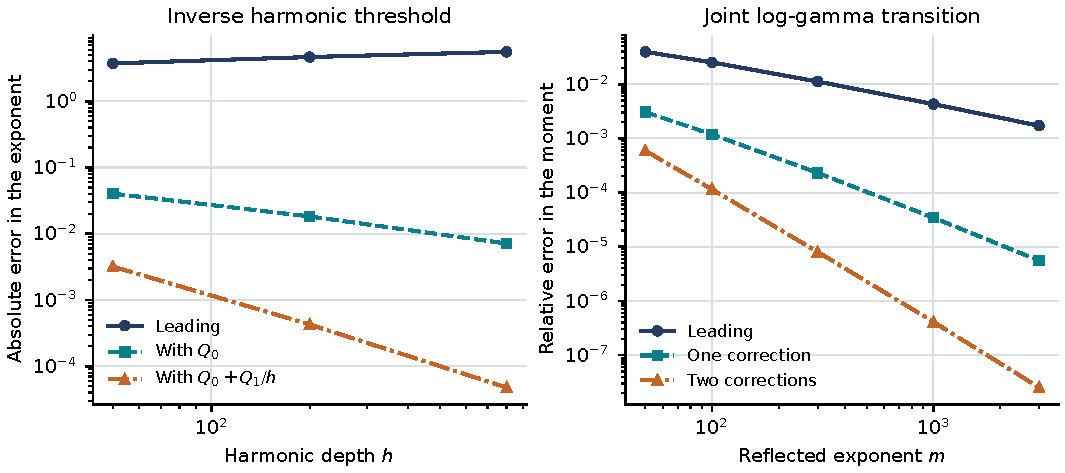
\includegraphics[width=\textwidth]{figures/correction_diagnostics.pdf}
\caption{Successive asymptotic corrections in the inverse harmonic
problem and the joint-moment transition. All plotted values are
high-precision diagnostics of the defining integrals. They are
distinct from the exact interval certificate used in the
monotonicity proof.}
\label{cont:fig:corrections}
\end{figure}

\subsection{Replay and portability}

Python 3.10 or later suffices for the supplied core scripts.
The symbolic and diagnostic programs additionally use SymPy and
mpmath; the versions used in this delivery are recorded in
\src{provenance/verification_receipt.json}. The package-level
\src{verify.py} runs the exact checks in a temporary directory,
compares the critical saved results, and records a fresh verification
receipt. Numerical diagnostics are available as an optional replay,
since they take longer and are not proof gates for the analytic
theorems. The \TeX{} source builds with a standard recent TeX Live
installation using \texttt{latexmk -pdf article.tex}.

The source receipts identify all thirty-nine inspected consolidated
source files and the six incoming archives. SHA-256 checksums cover
the delivered artifacts. These records make the scope of the audit
and the origin of the baseline unambiguous, without redistributing
the entire existing manuscript or its incoming packages.
